The reconnaissance phase focused on understanding the target application,
identifying exposed services and technologies, and mapping the observable
application attack surface before vulnerability assessment activities began.

\section{Objective}

The objective of this phase was to identify the target application, discover
its exposed network and application-level components, identify the technologies
in use, and collect information that could support the subsequent vulnerability
assessment.

The reconnaissance activities included technology identification, review of
accessible application information, port and service discovery, directory and
endpoint discovery, HTTP traffic analysis, and automated application crawling.
The tools used during this phase are listed in Table~\ref{tab:recon-tools}
in Chapter~3, Section~3.4.

\section{Target Identification}

The target application was confirmed to be accessible through the local
browser at \texttt{http://127.0.0.1:3000}. The application loaded successfully
and was available for subsequent reconnaissance and security testing.

\begin{figure}[H]
    \centering
    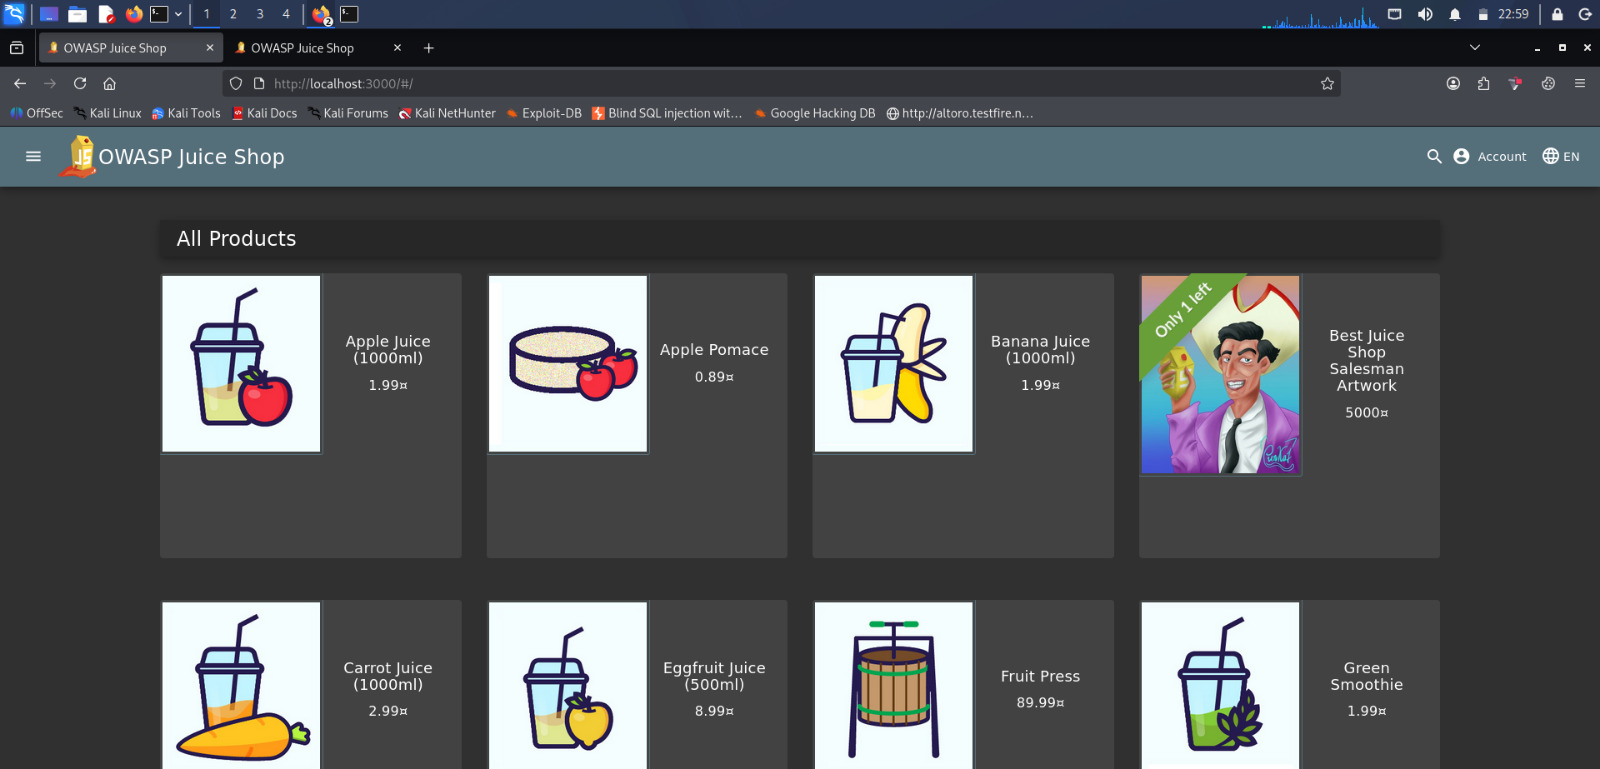
\includegraphics[width=0.90\textwidth]
    {evidence/phase2/images-proved/01-target-application.png}
    \caption{OWASP Juice Shop target application accessible at
    \texttt{http://127.0.0.1:3000}.}
    \label{fig:recon-target}
\end{figure}

\section{Port and Service Discovery}

Nmap was used to identify open ports and gather basic service information
from the target host. The scan identified port \texttt{3000/tcp} as open,
which was consistent with the locally hosted web application.

\begin{figure}[H]
    \centering
    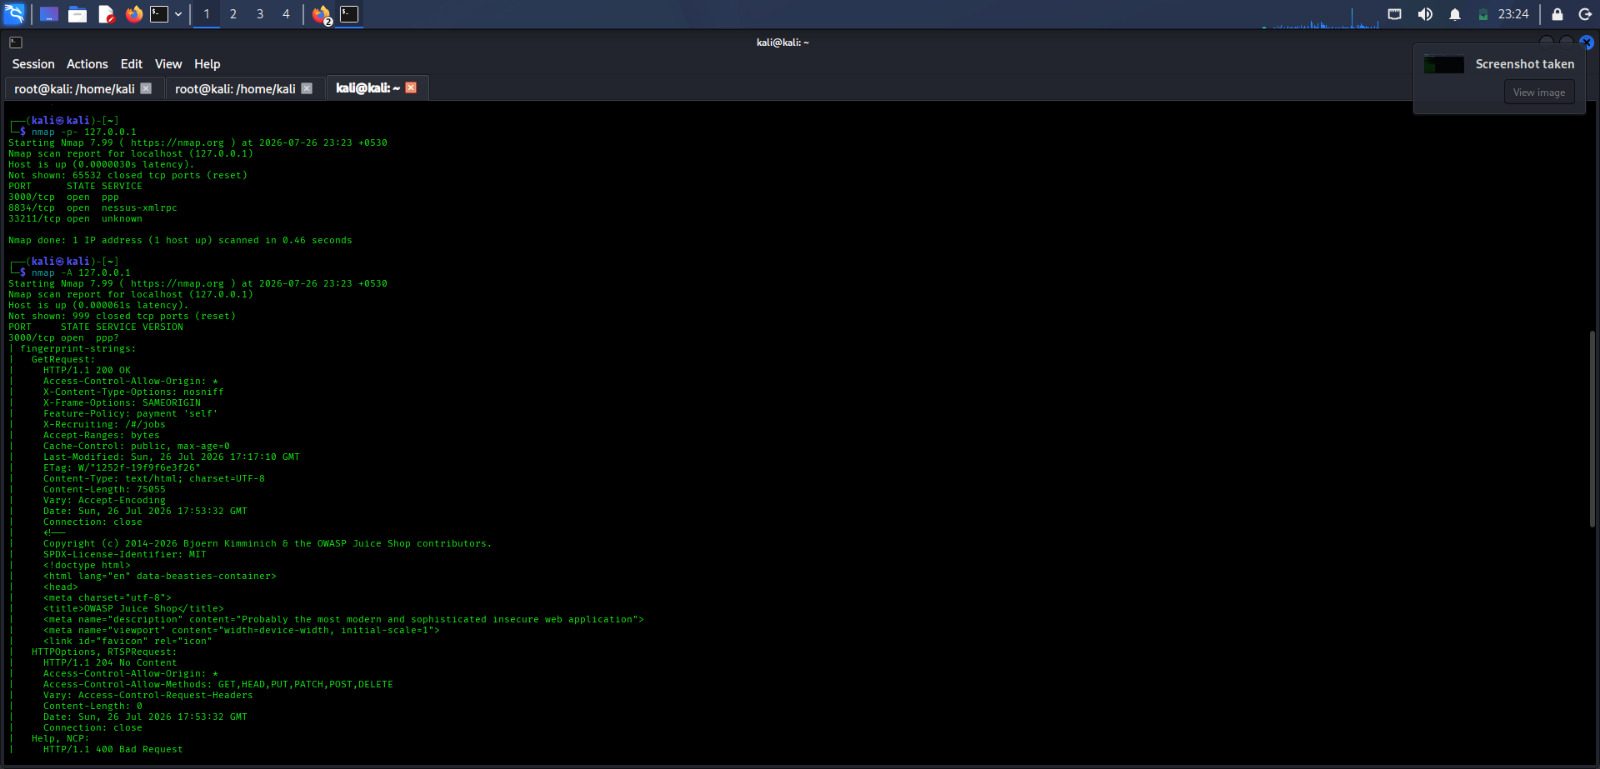
\includegraphics[width=0.90\textwidth]
    {evidence/phase2/images-proved/02-nmap-port-scan.png}
    \caption{Nmap port scan results showing port \texttt{3000/tcp} open.}
    \label{fig:recon-nmap-ports}
\end{figure}

A service-detection scan was also performed to gather additional information
about the service exposed on the identified port.

\begin{figure}[H]
    \centering
    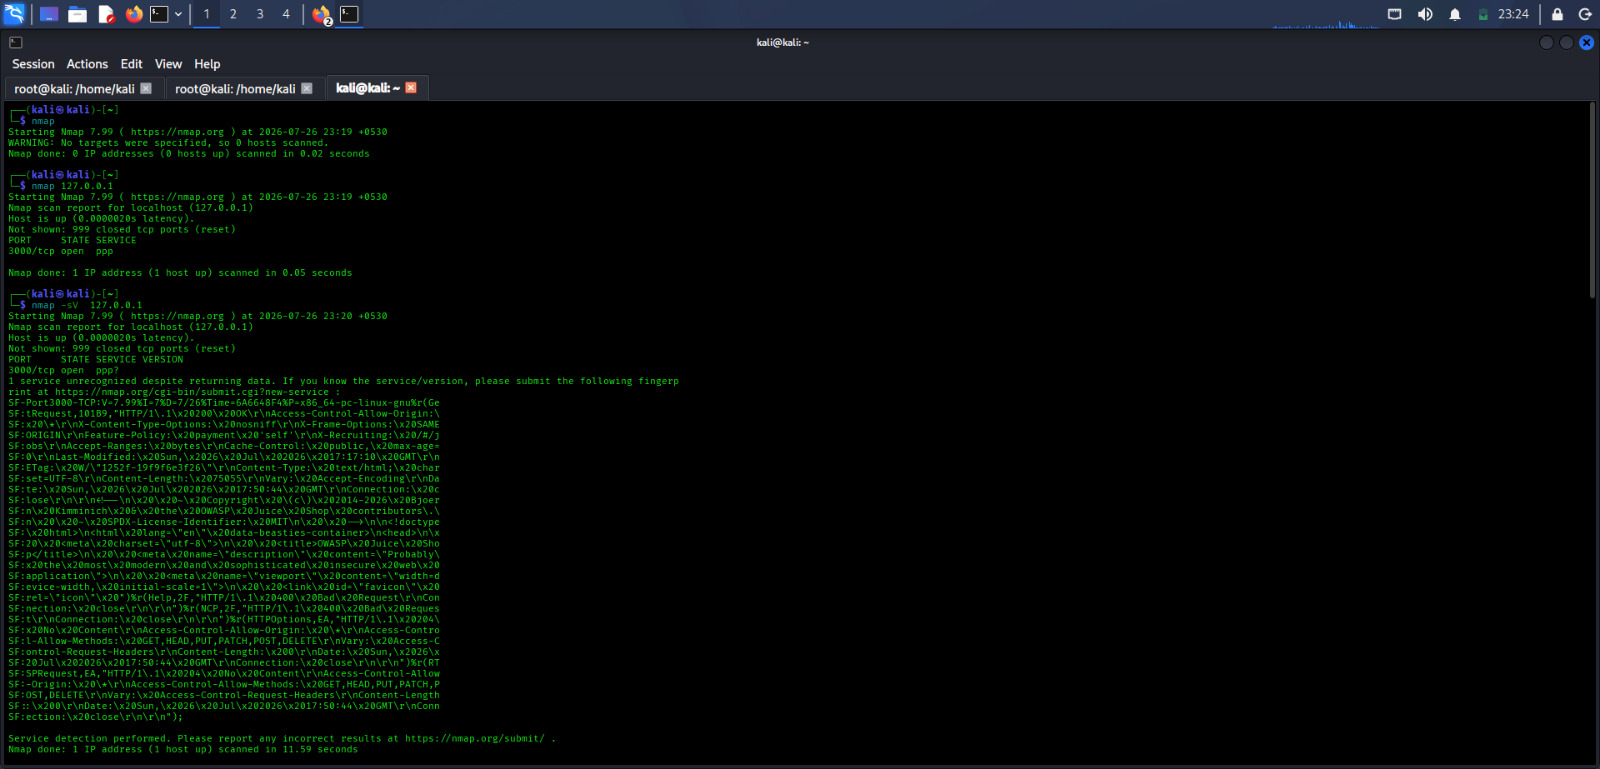
\includegraphics[width=0.90\textwidth]
    {evidence/phase2/images-proved/03-nmap-service-detection.png}
    \caption{Nmap service detection results for the identified web service.}
    \label{fig:recon-nmap-service}
\end{figure}

\section{Technology Identification}

Wappalyzer was used to identify technologies and frameworks associated with
the target application. The results provided information about the client-side
frameworks, libraries, content delivery services, and programming technologies
observed during reconnaissance.

\begin{figure}[H]
    \centering
    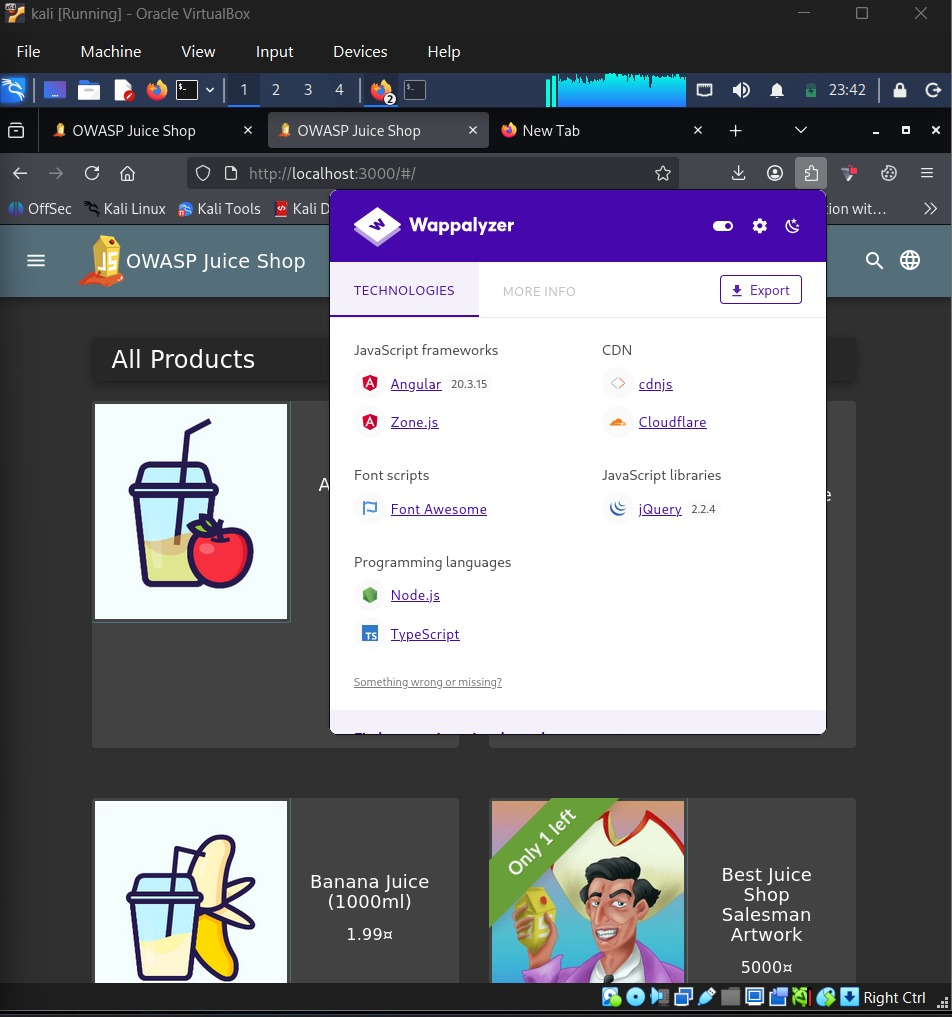
\includegraphics[width=0.85\textwidth]
    {evidence/phase2/images-proved/04-wappalyzer-technologies.png}
    \caption{Wappalyzer technology identification results.}
    \label{fig:recon-wappalyzer}
\end{figure}

\section{\texttt{robots.txt} Analysis}

The application's \texttt{robots.txt} file was directly accessed and reviewed
for path information that could reveal additional application resources.

The file contained a disallowed \texttt{/ftp} path, providing an additional
resource for reconnaissance and subsequent security testing.

\begin{figure}[H]
    \centering
    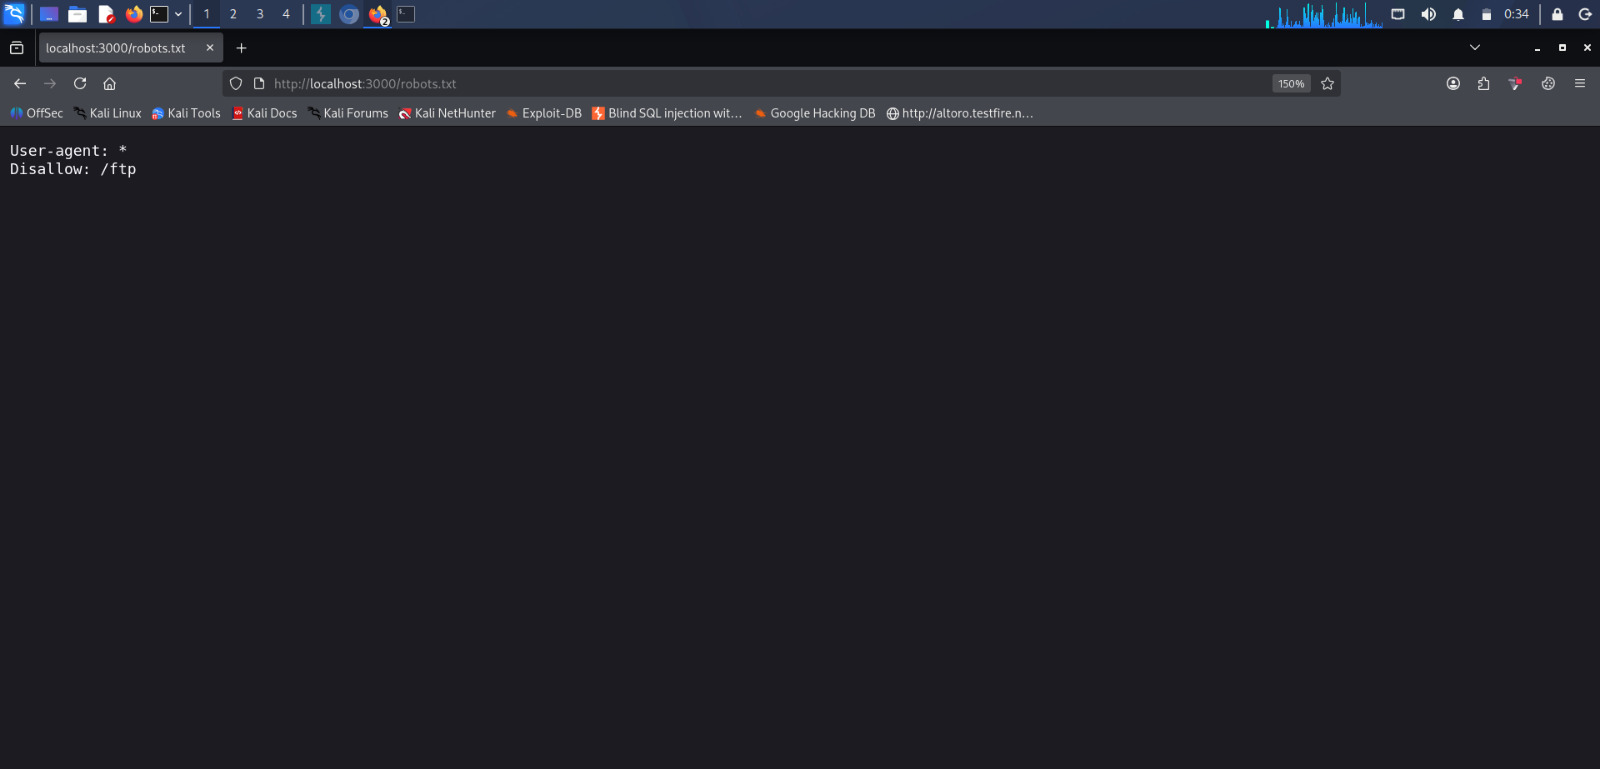
\includegraphics[width=0.90\textwidth]
    {evidence/phase2/images-proved/05-robots-txt.png}
    \caption{Contents of the application's \texttt{robots.txt} file.}
    \label{fig:recon-robots}
\end{figure}

\section{HTTP Request and Response Analysis}

Burp Suite was used as an intercepting proxy to observe HTTP communication
between the browser and the target application.

The captured traffic provided visibility into the HTTP methods, request
headers, cookies, target paths, and server responses. A successful
\texttt{HTTP/1.1 200 OK} response was observed for the captured request.

\begin{figure}[H]
    \centering
    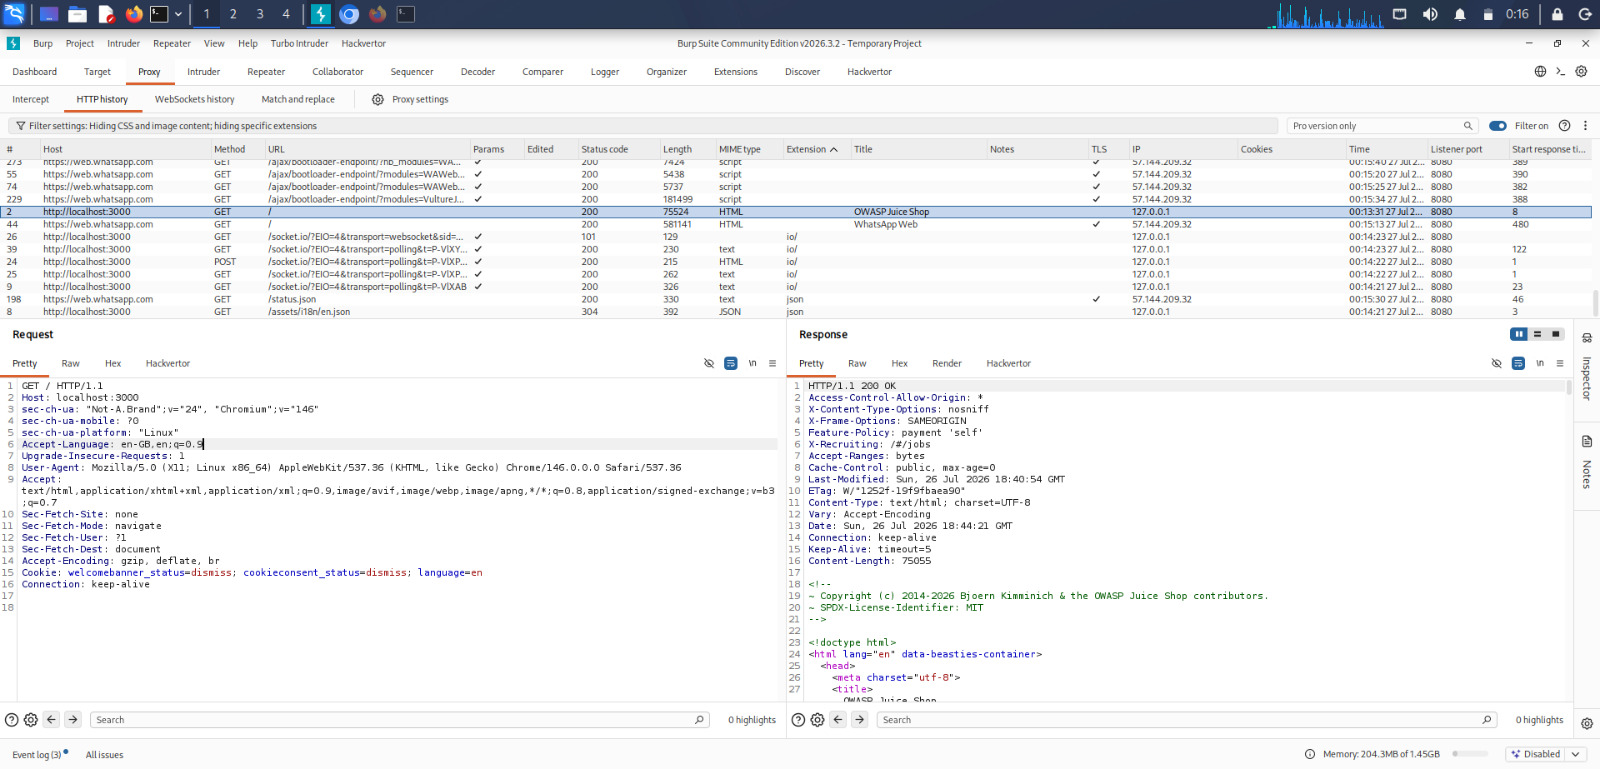
\includegraphics[width=0.95\textwidth]
    {evidence/phase2/images-proved/06-burp-http-request-response.jpeg}
    \caption{Burp Suite HTTP request and response captured during reconnaissance.}
    \label{fig:recon-burp}
\end{figure}

\section{Directory and Endpoint Discovery}

ffuf was used to perform active directory and endpoint discovery against the
target application. A commonly used web-content wordlist was used to identify
accessible paths that were not necessarily visible through normal application
navigation.

The scan identified multiple accessible paths, including examples such as
\texttt{/api}, \texttt{/ftp}, \texttt{/rest}, \texttt{/assets}, and
\texttt{/robots.txt}.

\begin{figure}[H]
    \centering
    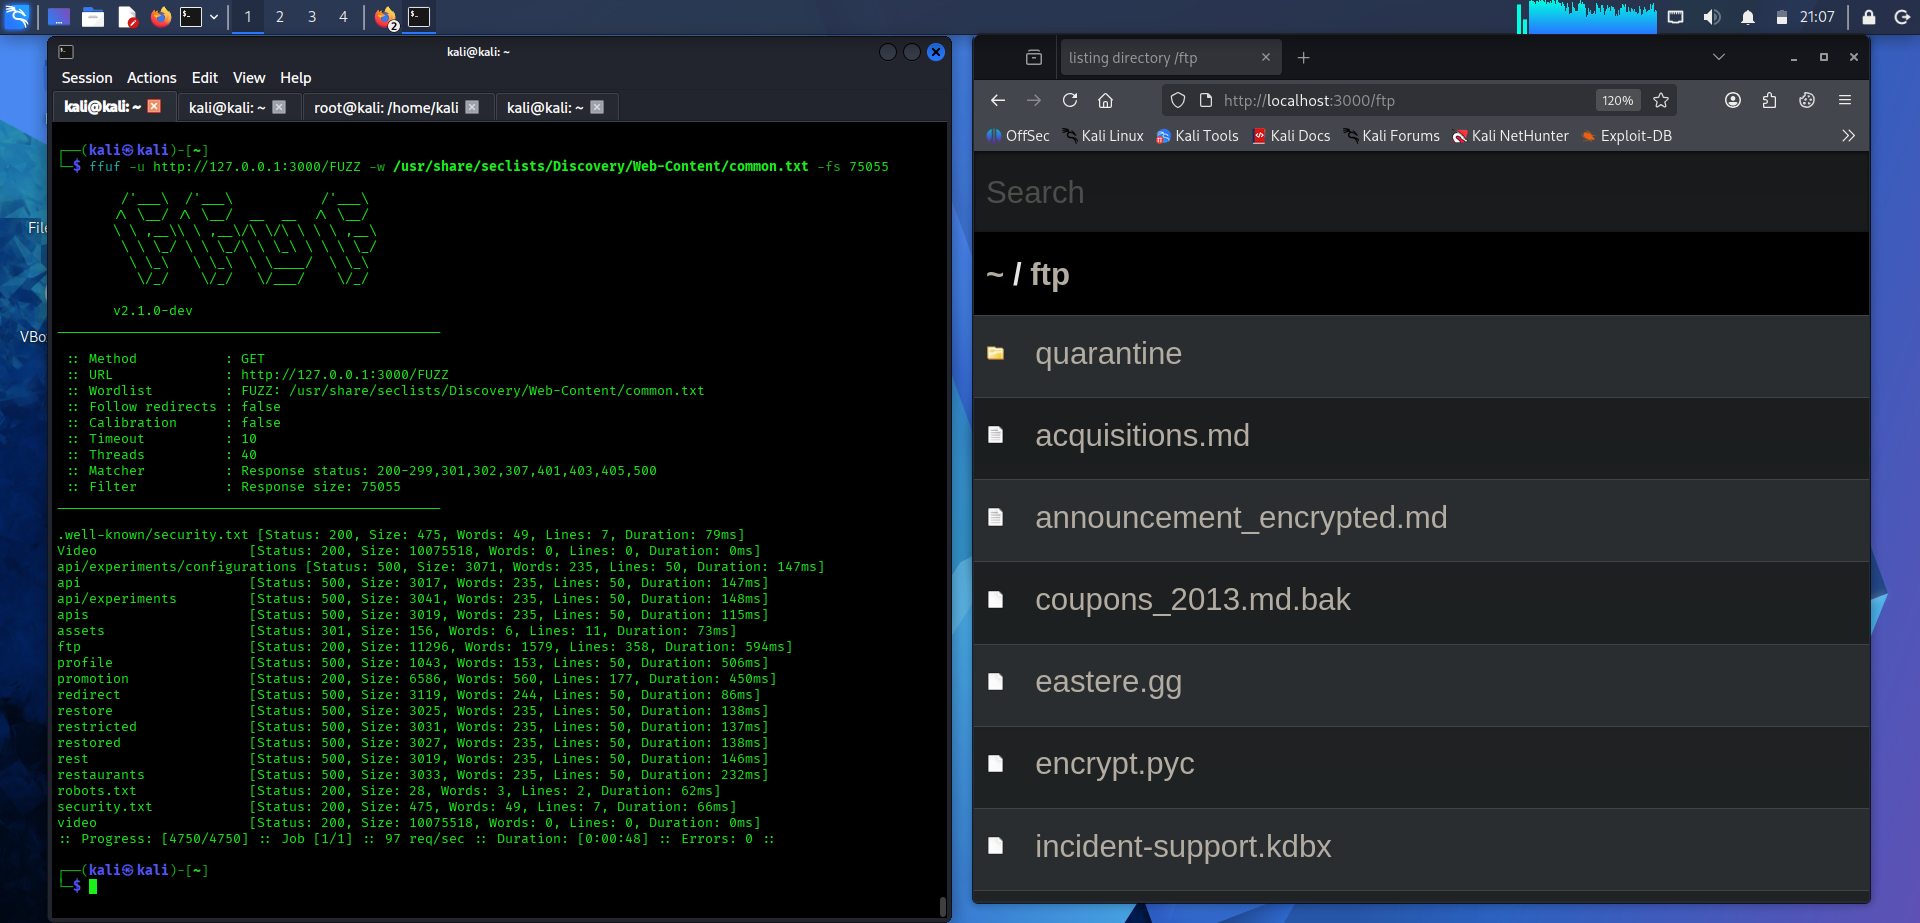
\includegraphics[width=0.90\textwidth]
    {evidence/phase2/images-proved/07-ffuf-directory-discovery.png}
    \caption{ffuf directory and endpoint discovery results.}
    \label{fig:recon-ffuf}
\end{figure}

\section{OWASP ZAP Spider}

The OWASP ZAP Spider was used to automatically crawl the target application
and identify reachable resources and links.

The completed Spider scan reported:

\begin{itemize}
    \item \textbf{URLs Found:} 398
    \item \textbf{Nodes Added:} 255
\end{itemize}

The crawl identified a number of application resources and REST-style
endpoints that expanded the observable attack surface.

\begin{figure}[H]
    \centering
    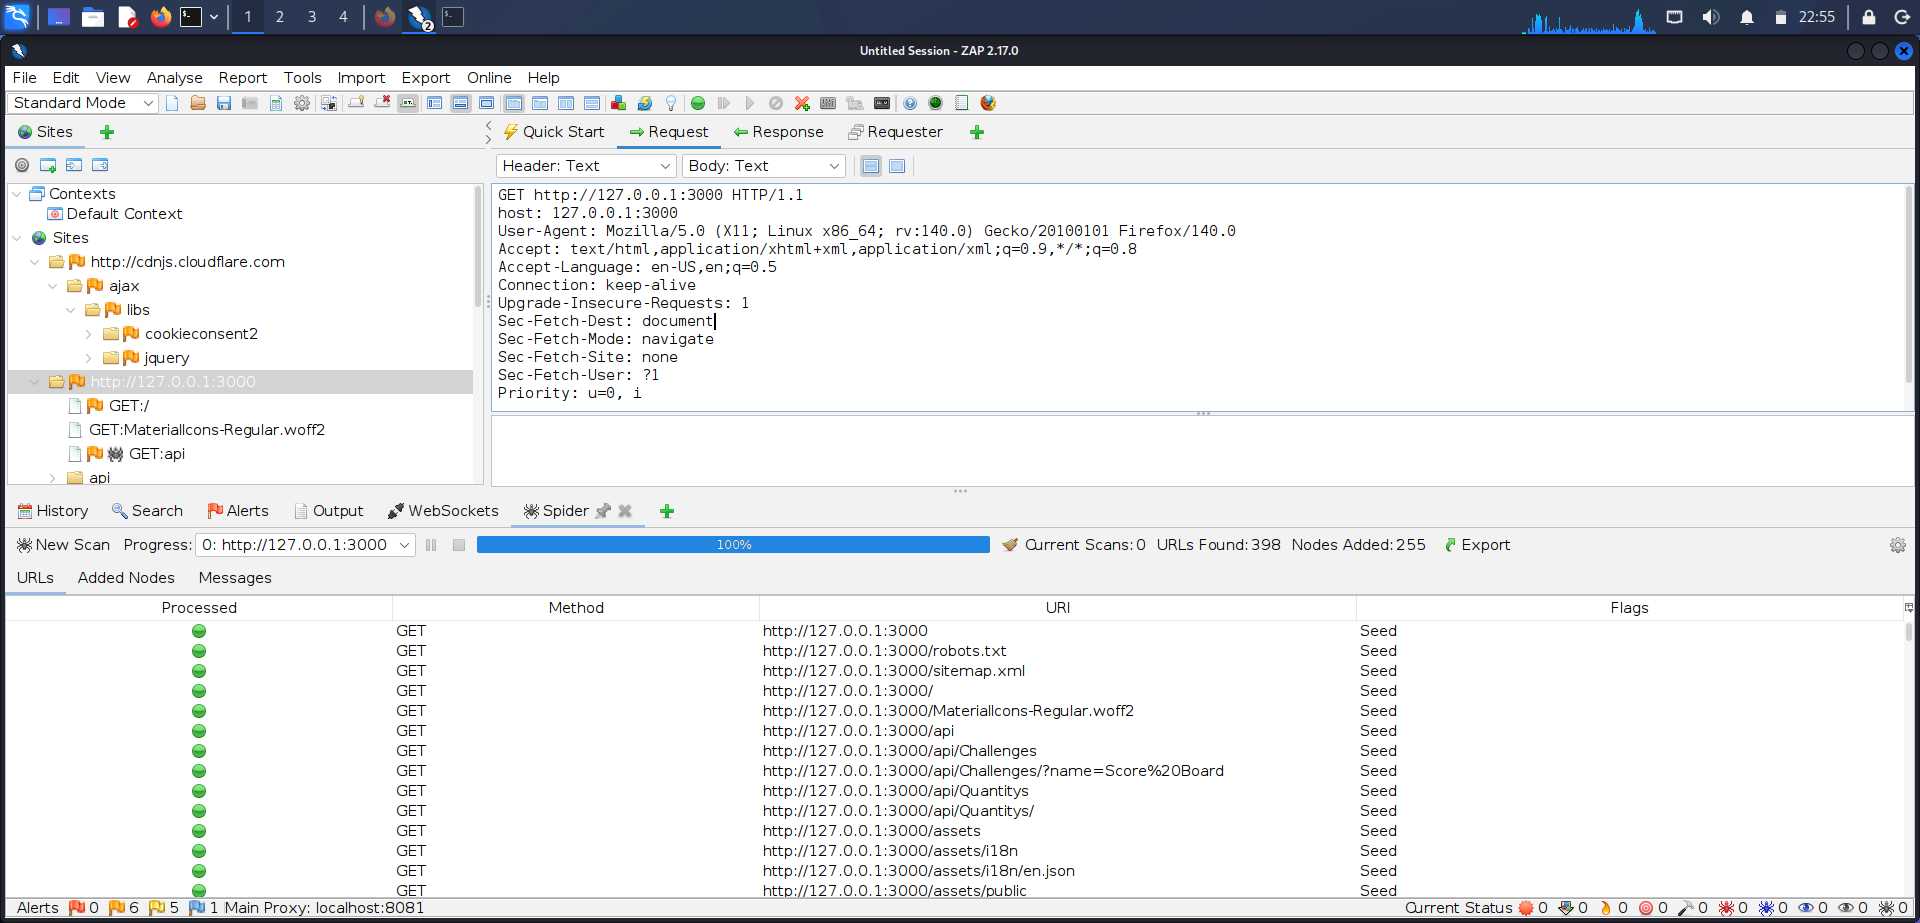
\includegraphics[width=0.95\textwidth]
    {evidence/phase2/images-proved/08-zap-spider-results.png}
    \caption{OWASP ZAP Spider results showing 398 URLs found and 255 nodes added.}
    \label{fig:recon-zap-spider}
\end{figure}

\section{OWASP ZAP AJAX Spider}

The OWASP ZAP AJAX Spider was additionally used to crawl the application through
browser-based navigation and identify resources and routes associated with
client-side application behavior.

The completed AJAX Spider scan reported:

\begin{itemize}
    \item \textbf{URLs Crawled:} 383
\end{itemize}

The AJAX crawl provided additional visibility into dynamically requested
resources and JavaScript-driven application behavior.

\begin{figure}[H]
    \centering
    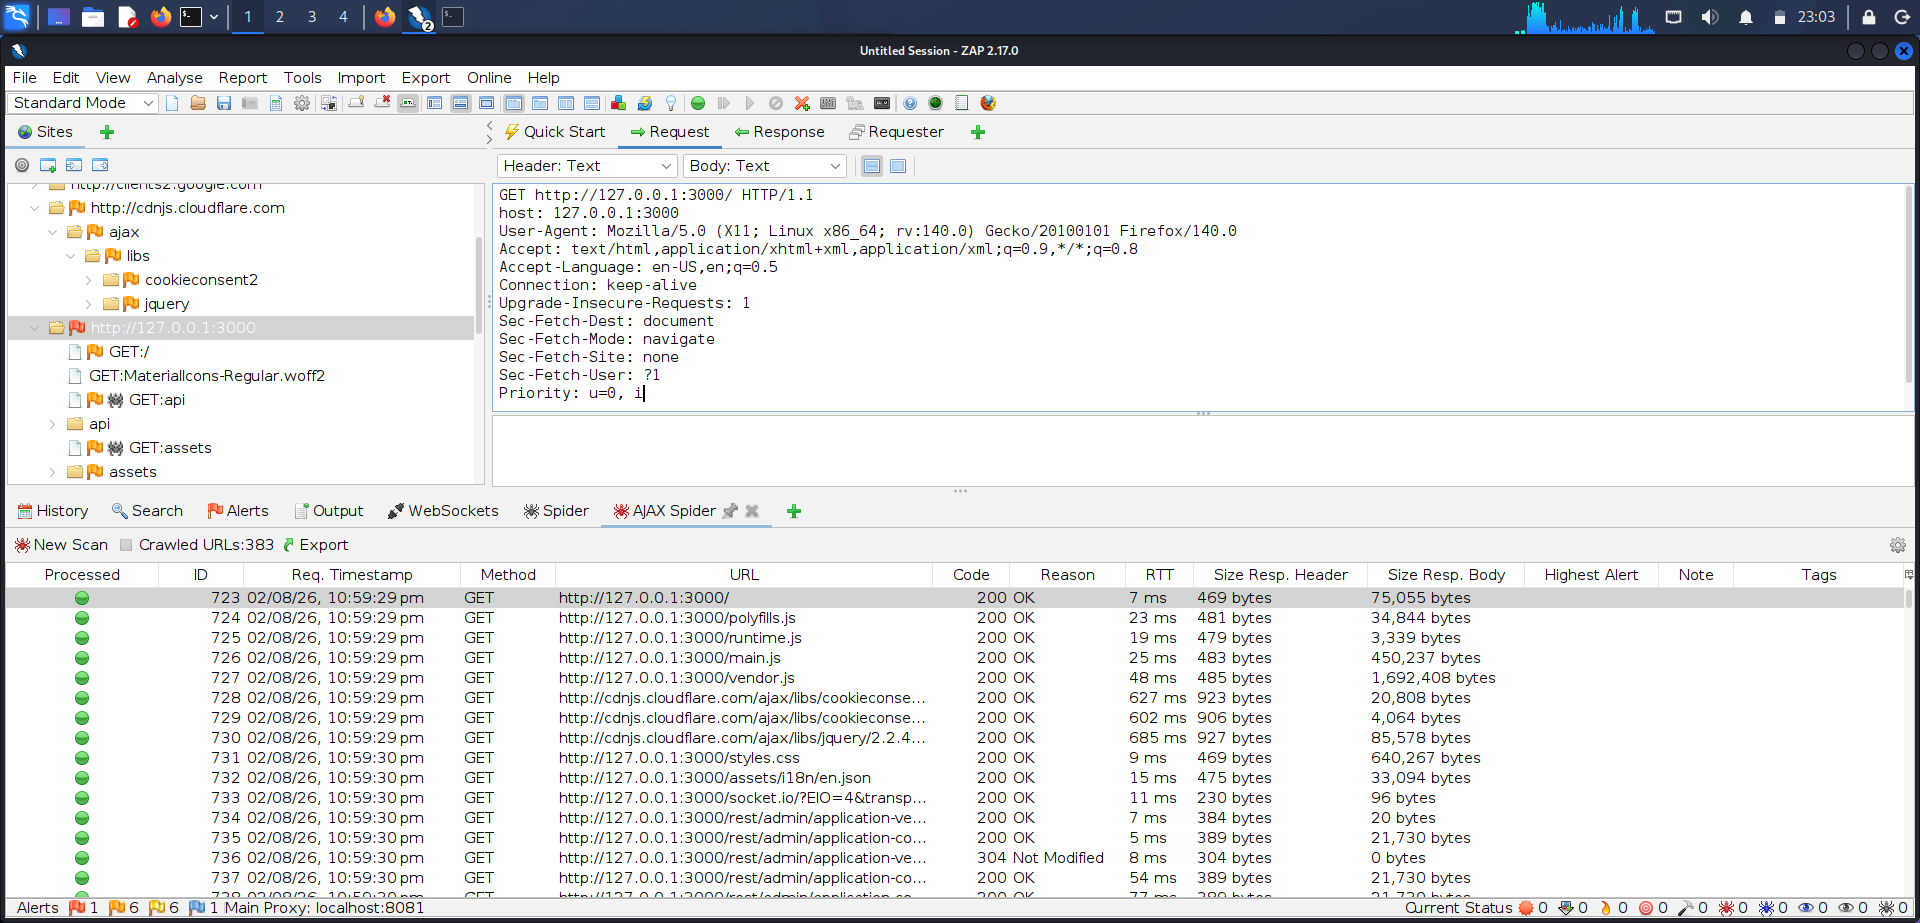
\includegraphics[width=0.95\textwidth]
    {evidence/phase2/images-proved/09-zap-ajax-spider-results.png}
    \caption{OWASP ZAP AJAX Spider results showing 383 URLs crawled.}
    \label{fig:recon-zap-ajax}
\end{figure}

\section{Reconnaissance Summary}

The reconnaissance activities established an initial view of the application's
observable attack surface.

The target was confirmed to be accessible at
\texttt{http://127.0.0.1:3000}, and Nmap identified port
\texttt{3000/tcp} as open. Wappalyzer identified multiple technologies and
frameworks associated with the application.

The review of \texttt{robots.txt} revealed the \texttt{/ftp} path, while ffuf
identified additional application paths and resources. Burp Suite provided
visibility into HTTP request and response behavior. OWASP ZAP further expanded
the observable application map through both traditional and AJAX-based
crawling.

The information collected during this phase was used to guide vulnerability
scanning and assessment activities in Phase 3 and manual verification and
proof-of-concept testing in Phase 4.

\begin{table}[H]
\centering
\begin{tabularx}{\textwidth}{>{\bfseries}p{0.38\textwidth} X}
\toprule
Metric & Result \\
\midrule
Target &
\texttt{http://127.0.0.1:3000} \\

Open Port Identified &
\texttt{3000/tcp} \\

ffuf Discovery &
Multiple accessible paths identified \\

ZAP Spider &
398 URLs / 255 nodes \\

ZAP AJAX Spider &
383 URLs crawled \\

\texttt{robots.txt} Observation &
\texttt{/ftp} path disclosed \\

HTTP Analysis &
Successful \texttt{HTTP/1.1 200 OK} response observed \\
\bottomrule
\end{tabularx}
\caption{Reconnaissance phase summary}
\label{tab:recon-summary}
\end{table}

\section{Phase 3 Preparation}

The reconnaissance results established the initial attack surface that was
used to guide Phase 3 vulnerability scanning and assessment activities.

A complete de-duplicated endpoint inventory is not included in this section
until the raw ffuf, ZAP Spider, and AJAX Spider outputs have been consolidated.
This avoids presenting a partial endpoint list as a complete inventory.